% Junior Level 3, Week 8 -- play-at-home card
\homeworkweek{8}{Colors and My Own Pattern}{Optional. One short game with a grown-up.}

\begin{playathome}[Color by code]
The color key is a tiny program. Color the grid with it.
\begin{center}
\begin{tabular}{@{}l@{}}
\texttt{1 = "gold"}\\
\texttt{2 = "blue"}
\end{tabular}
\qquad
%% alt: A 4 by 4 grid of empty squares with a number in each. Row 1: 1, 2, 2, 1. Row 2: 2, 1, 1, 2. Row 3: 2, 1, 1, 2. Row 4: 1, 2, 2, 1.
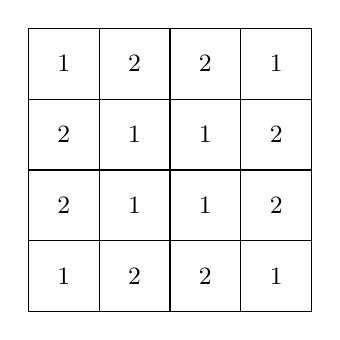
\begin{tikzpicture}[baseline=(current bounding box.center)]
  \foreach \row/\vals in {0/{1,2,2,1},1/{2,1,1,2},2/{2,1,1,2},3/{1,2,2,1}} {
    \foreach \v [count=\col] in \vals {
      \draw (\col*0.9,-\row*0.9) rectangle ++(0.9,0.9);
      \node[font=\small] at (\col*0.9+0.45,-\row*0.9+0.45) {\v};
    }
  }
\end{tikzpicture}
\end{center}
\begin{enumerate}[leftmargin=1.4em,itemsep=2pt]
  \item Color every 1 gold and every 2 blue.
  \item Remix it! Pick new colors for 1 and 2. Draw the grid again and color it.
  \item Write on your remix: \enquote{Idea from: Kids Coding. Remixed by:} and your nickname.
\end{enumerate}
\end{playathome}

\begin{playathome}[If you have Thonny at home]
Open your flower. Try \texttt{t.pensize(10)}. Run it. Is it too thick, or the right size?
\end{playathome}

\begin{selfcheck}
  \item I changed a color and the pen size in Python.
  \item I can say what a remix is and why we give credit.
\end{selfcheck}
